\section{Editor}

Di seguito viengono elencati i casi d'uso per l'editor.

%\newpage da rimuovere?

\subsection{Casi d'Uso}


\subsubsection{UC-E}

    \begin{figure}[H]
      \begin{center}
        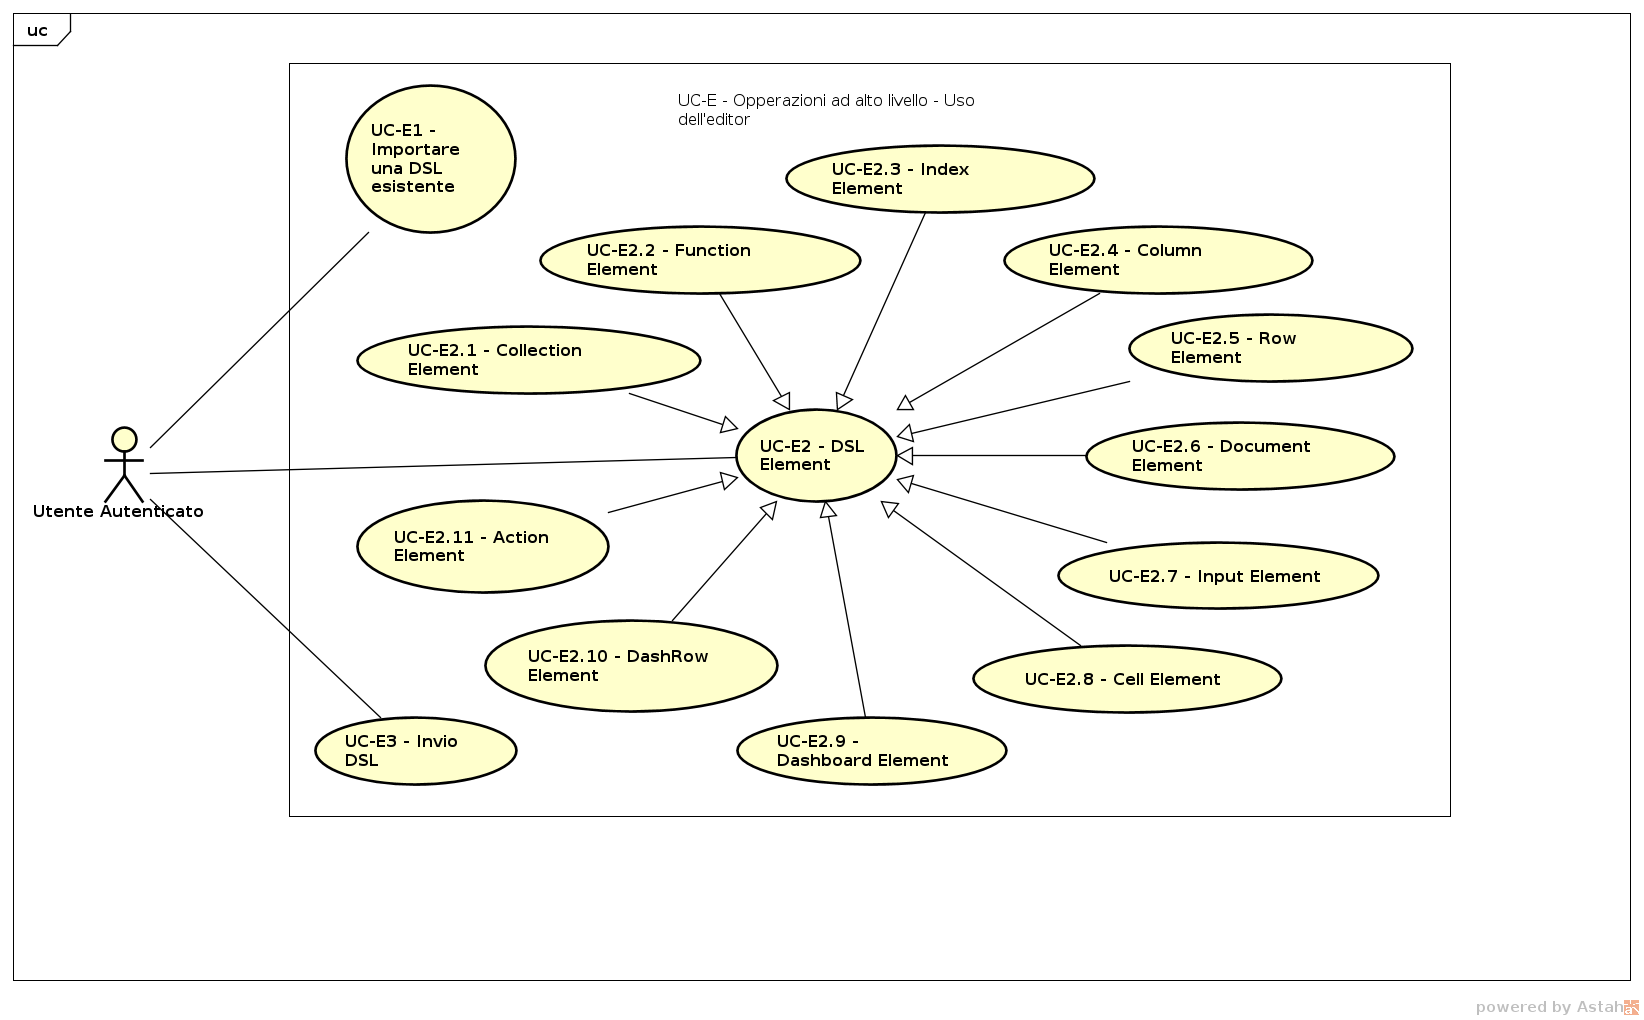
\includegraphics[width=12cm]{res/img/UCEditor/UC-E}
      \caption{UC-E - Operazioni ad alto livello - Uso dell'editor}
      \end{center} 
    \end{figure}    
    
    %Tabella 
    \begin{center}
      \bgroup
      \def\arraystretch{1.8}     
      \begin{longtable}{  p{3.5cm} | p{8cm} } 
        
        \hline
        \multicolumn{2}{ | c | }{ \cellcolor[gray]{0.9} \textbf{UC-E - Operazioni ad alto livello - Uso dell'editor}} \\ 
        \hline
        
        \textbf{Attori Primari} & Utente Autenticato, Ospite, Membro, Admin, Proprietario \\ 
        \textbf{Scopo e Descrizione} & 1. Importare un DSL esitente (UC-E1)
2. Manipolazione del DSL Element tramite l'interfaccia grafica dell'editor
3. Invio del DSL \\ 
        
        \textbf{Precondizioni}  & 1. Importare un DSL esitente (UC-E1)
2. Manipolazione del DSL Element tramite l'interfaccia grafica dell'editor
3. Invio del DSL \\ 
        
        \textbf{Postcondizioni} & L'utente ha utilizzato l'editor ed ha eseguito le azioni volute \\ 
        \textbf{Flusso Principale} & 1. Importare un DSL esistente
2. DSL element
3. Invio di un DSL \\
        \textbf{Estensioni} &  \\
        \textbf{Inclusioni} & 
      \end{longtable}
      \egroup
    \end{center} 


\subsubsection{UC-E2}

    \begin{figure}[H]
      \begin{center}
        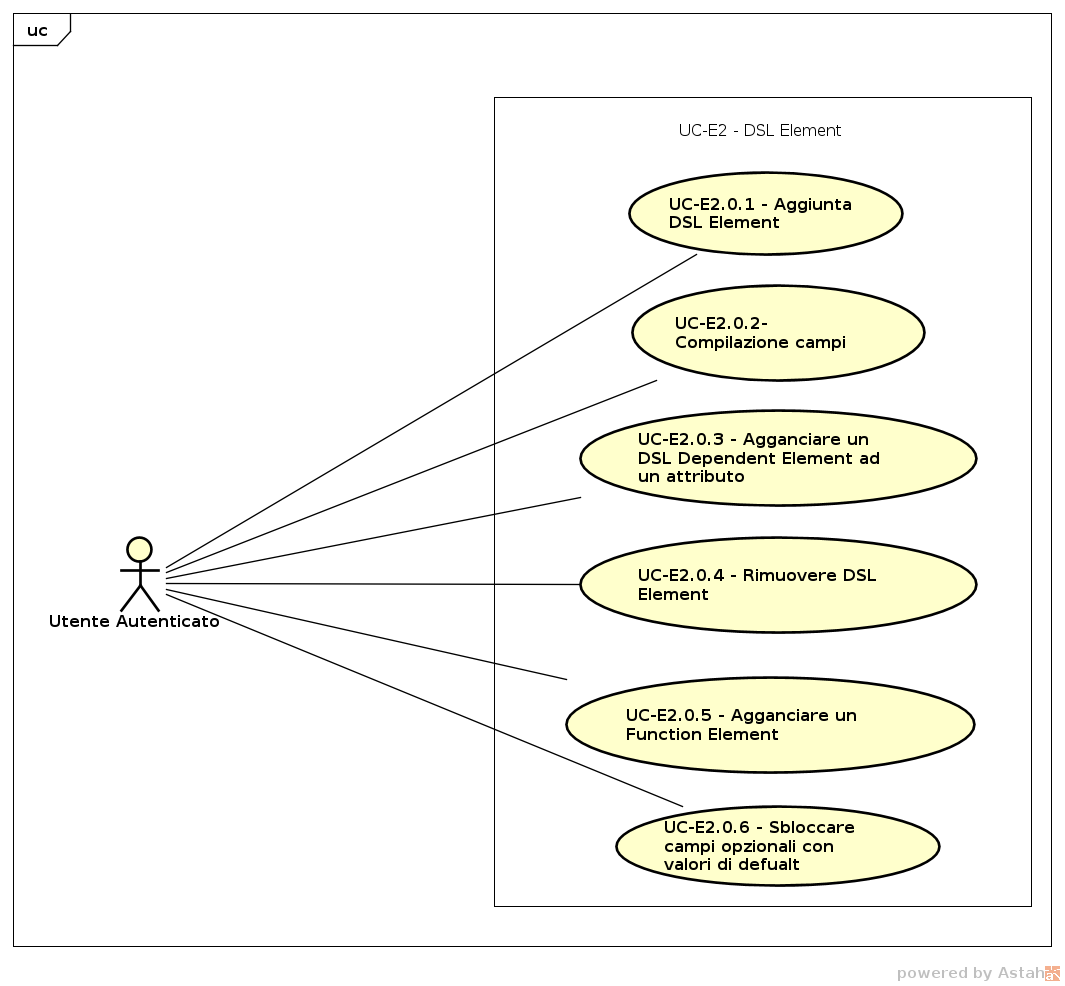
\includegraphics[width=12cm]{res/img/UCEditor/UC-E2-DSLElement}
      \caption{UC-E2 - DSL Element}
      \end{center} 
    \end{figure}    
    
    %Tabella 
    \begin{center}
      \bgroup
      \def\arraystretch{1.8}     
      \begin{longtable}{  p{3.5cm} | p{8cm} } 
        
        \hline
        \multicolumn{2}{ | c | }{ \cellcolor[gray]{0.9} \textbf{UC-E2 - DSL Element}} \\ 
        \hline
        
        \textbf{Attori Primari} & Utente Autenticato, Ospite, Membro, Admin, Proprietario \\ 
        \textbf{Scopo e Descrizione} & Il DSL element è la zona dove è possibile aggiungere, agganciare, sbloccare o rimuovere altri elementi del DSL. È possibile anche la compilazione dei campi. \\ 
        
        \textbf{Precondizioni}  & Il DSL element è la zona dove è possibile aggiungere, agganciare, sbloccare o rimuovere altri elementi del DSL. È possibile anche la compilazione dei campi. \\ 
        
        \textbf{Postcondizioni} & L'utente ha eseguito le sue operazioni sul DSL Element \\ 
        \textbf{Flusso Principale} & 1. Aggiunta DSL Element (UC-E2.0.1)
2. Compilazione campi (UC-E2.0.2)
3. Agganciare un DSL Dependent Element ad un attributo (UC-E2.0.3)
4. Rimuovere DSL Element (UC-E2.0.4)
5. Agganciare un Function Element (UC-E2.0.5)
6. Sbloccare campi opzionali con valori di default (UC-E2.0.6) \\
        \textbf{Estensioni} &  \\
        \textbf{Inclusioni} & 
      \end{longtable}
      \egroup
    \end{center} 


\subsubsection{UC-E2.0.1}

    %\begin{figure}[H]
    %  \begin{center}
    %    \includegraphics[width=12cm]{res/img/}
    %  \caption{UC-E2.0.1 - Aggiunta DSL Element}
    %  \end{center} 
    %\end{figure}    
    
    %Tabella 
    \begin{center}
      \bgroup
      \def\arraystretch{1.8}     
      \begin{longtable}{  p{3.5cm} | p{8cm} } 
        
        \hline
        \multicolumn{2}{ | c | }{ \cellcolor[gray]{0.9} \textbf{UC-E2.0.1 - Aggiunta DSL Element}} \\ 
        \hline
        
        \textbf{Attori Primari} & Utente Autenticato, Ospiete, Membro, Admin, Proprietario \\ 
        \textbf{Scopo e Descrizione} & L'utente ha la possibiltà di aggiungere un elemento DSL \\ 
        
        \textbf{Precondizioni}  & L'utente ha la possibiltà di aggiungere un elemento DSL \\ 
        
        \textbf{Postcondizioni} & L'utente ha aggiunto con successo un elemento DSL \\ 
        \textbf{Flusso Principale} &  \\
        \textbf{Estensioni} &  \\
        \textbf{Inclusioni} & 
      \end{longtable}
      \egroup
    \end{center} 
